\documentclass{ctexart}
\usepackage{Note}
\begin{document}
\section{几何处理}
\subsection{几何操作的数学基础}
\subsection{离散微分几何}
我们总是用离散的网格\footnote{在本节,我们主要以三角网格作为研究对象.}来描述连续的曲面,但网格定义出的几何形状只能给出$\mathcal{C}^0$连续性.如何将连续曲面的各种微分量应用在离散的情况下就属于\tbf{离散微分几何}研究的内容.常见的各种微分量有法向量,曲率,拉普拉斯算子等.
\subsubsection{局部平均区域}
我们可以用下面的方法刻画三角网格顶点$\vec{x}_i$处的微分量$\vec{f}$:
\[\vec{f}\left(\vec{x}_i\right)=\left(\displaystyle\iint_{\Omega\left(\vec{x}_i\right)}\vec{f}\di S\right)\Big/\left(\displaystyle\iint_{\Omega\left(\vec{x}_i\right)}\di S\right)\]
即在$\vec{x}$的某个邻域$\Omega(\vec{x})$的邻域上该微分量的平均值.邻域的选择直接影响离散微分量的结果和准确度.邻域越大,结果越平滑,但也会丢失更多的细节.邻域越小,结果越接近真实值,但也对噪声更敏感.常见的邻域选择有以下几种:
\begin{enumerate}[label=\tbf{\arabic*.},topsep=0pt,parsep=0pt,itemsep=0pt,partopsep=0pt]
    \item \tbf{重心单元(barycentric cell)}:把与顶点$\vec{x}$相邻的所有三角形的两边的中点和重心连起来形成的多边形区域.
    \item \tbf{泰森多边形单元(Voronoi cell)}:把与顶点$\vec{x}$相邻的所有三角形的外心连起来形成的多边形区域.
    \item \tbf{混合泰森多边形单元(mixed Voronoi cell)}: Vorinoi cell在钝角三角形中取的点可能超出三角形外,因此在钝角三角形中用边的中点代替外心,其余情形不变.
\end{enumerate}
\subsubsection{法向量}
三角形内部点的法向量可以唯一地定义为三角形所在平面的法向量.对于顶点$\vec{x}$处的法向量$\vec{n}(\vec{x})$,可以通过对顶点周围三角形的法向量加权平均得到:
\[\vec{n}(\vec{x})=\dfrac{\displaystyle\sum_{T\in\Omega(\vec{x})}\alpha_T\vec{n}(T)}{\displaystyle\sum_{T\in\Omega(\vec{x})}\alpha_T\left|\left|\vec{n}(T)\right|\right|}\]
其中$\Omega(\vec{x})$是与顶点$\vec{x}$邻接的三角形构成的几何,$\alpha_T$和$\vec{n}(T)$是三角形$T$的权重和法向量.常见的权重有以下几种:
\begin{enumerate}[label=\tbf{\arabic*.},topsep=0pt,parsep=0pt,itemsep=0pt,partopsep=0pt]
    \item \tbf{常数权重}: $\alpha_T=1$.这在计算上最简单,但对于一些不规则网格效果不好.
    \item \tbf{面积权重}: $\alpha_T=A_T$.以三角形面积$A_T$加权,比常数权重更合理,但对过于不规则的网格效果也不好.
    \item \tbf{角度权重}: $\alpha_T=\theta_T$,其中$\theta_T$是顶点$\vec{x}$在三角形$T$中的对角.这样加权效果最好,但计算上也最复杂.
\end{enumerate}
\subsubsection{梯度}
梯度是非常重要的微分量,在计算拉普拉斯算子,网格参数化等方面有重要应用.\\
\indent 对于一个在三角网格上定义的标量函数$f$,我们可以通过$f$在三角形顶点上的值通过重心插值的方式得到三角形内部的值.不妨设三角形的顶点为$\vec{x}_a,\vec{x}_b,\vec{x}_c$,则其内部任意一点$\vec{x}$的值为:
\[f(\vec{x})=\alpha(\vec{x})f(\vec{x}_a)+\beta(\vec{x})f(\vec{x}_b)+\gamma(\vec{x})f(\vec{x}_c)\]
其中$\alpha,\beta,\gamma$是点$\vec{x}$在三角形中的重心坐标,在\tbf{Lecture 3 绘图}一节中已经讲过其定义方式.我们在那时已经证明重心坐标是线性的,因此$f$的梯度$\nabla f$也是定值.现在来证明之.
\begin{proof}
    不妨假定$\vec{x}_a,\vec{x}_b$和$\vec{x}_c$在三角形$T$中对应的顶点分别为$A,B$和$C$, $\vec{x}$对应$T$内的一点$P$.以$\alpha(\vec{x})$为例,根据重心坐标与三角形面积的关系,有
    \[\alpha(\vec{x})=\dfrac{A_{\triangle PBC}}{A_{\triangle ABC}}=\dfrac{\overline{BP}\cdot\overline{BC}\cdot\sin\angle PBC}{2A_T}=\dfrac{\left|\left|\overrightarrow{BP}\times\overrightarrow{BC}\right|\right|}{2A_T}=\dfrac{\left(\vec{x}-\vec{x}_b\right)\cdot\left(\vec{x}_c-\vec{x}_b\right)^{\bot}}{2A_T}\]
    其中$\left(\vec{x}_c-\vec{x}_b\right)^\bot$表示该向量在平面上逆时针旋转$90^\circ$后的向量.于是
    \[\nabla\alpha(\vec{x})=\dfrac{\left(\vec{x}_c-\vec{x}_b\right)^\bot}{2A_T}\]
    于是
    \[\nabla f(\vec{x})=\dfrac{\left(\vec{x}_c-\vec{x}_b\right)^\bot}{2A_T}f\left(\vec{x}_a\right)+\dfrac{\left(\vec{x}_a-\vec{x}_c\right)^\bot}{2A_T}f\left(\vec{x}_b\right)+\dfrac{\left(\vec{x}_b-\vec{x}_a\right)^\bot}{2A_T}f\left(\vec{x}_c\right)\]
    这表明$\nabla f(\vec{x})$与$\vec{x}$无关,即在三角形内部为常值.
\end{proof}
\subsubsection{离散拉普拉斯算子}
\begin{definition}[拉普拉斯算子]
    \tbf{拉普拉斯算子(Laplace Operator, Laplacian)}是一个二阶微分算子,记号为$\Delta$或$\nabla^2$,定义为函数梯度的散度:
    \[\Delta f=\text{div}\left(\text{grad}\ f\right)\]
    在$n$维欧氏空间中,对于一个标量函数$f\left(\li x,n\right)$,拉普拉斯算子可以表示为:
    \[\Delta=\sum_{i=1}^{n}\dfrac{\p^2}{\p x_i^2}\]
\end{definition}
我们知道,对于一维函数,其二阶导数表示该函数的凹凸程度;而Laplacian是多维函数在各个正交的方向上的二阶导数之和,也就刻画了该函数在某一点整体的凹凸程度.\\
\indent 我们也可以用梯度和散度的几何意义理解Laplacian.梯度作为向量场衡量了函数在各点的变化方向,再对其求散度就可以得到函数在该点附近梯度的情况.如果梯度场\textit{流入}某一点更多,此时该点的Laplacian为正,表明此处函数内凹(类似于山谷);反之,如果梯度场\textit{流出}某一点更多,此时该点的Laplacian为负,表明此处函数外凸(类似于山峰).当梯度场流入和流出的量近似时,该点的Laplacian接近零,表明此处函数比较平坦\footnote{这里的平坦不是指函数值变化不大,而是指函数值的变化速率变化不大,类似于一次函数.}(类似于山坡).\\
\indent Laplacian对于刻画曲面性质有重要作用.例如,我们可以用Laplacian计算由参数方程$\vec{S}(u,v)$在三维空间中定义的曲面$S$的平均曲率\footnote{对于一个曲面$S$上某一点$P$,过$P$的法向量做平面可以与$S$交出一条曲线$C$.改变平面的方向所得的$C$中在$P$处的曲率有极大值$k_1$和极小值$k_2$,称作曲面$S$在点$P$处的\tbf{主曲率}(Principal Curvature).曲面$S$在$P$处的\tbf{平均曲率}(Mean Curvature)定义为$H=\left(k_1+k_2\right)/2$.以后也许还会用到\tbf{高斯曲率}(Gaussian Curvature),定义为$K=k_1k_2$.}:
\[H=-\dfrac{\Delta\vec{S}}{2\vec{n}}\]
\indent 在离散情况下,我们可以得到如下结论.
\begin{definition}[离散拉普拉斯算子]
    在三角形网格中,函数$f$在顶点$\vec{x}_i$处的\tbf{离散拉普拉斯算子(Discrete Laplace Operator)}定义为:
    \[\Delta f\left(\vec{x}_i\right)=\sum_{\vec{x}_j\in\Omega(\vec{x}_i)}w_{ij}\left(f\left(\vec{x}_j\right)-f\left(\vec{x}_i\right)\right)\]
    其中$\Omega(\vec{x}_i)$是与顶点$\vec{x}_i$邻接的顶点集合, $w_{ij}$是权重.
\end{definition}
\begin{definition}[均匀拉普拉斯算子]
    \tbf{均匀拉普拉斯算子(Uniform Laplace Operator)}的权重定义为:
    \[w_{ij}=\dfrac{1}{\left|\Omega(\vec{x}_i)\right|}\]
    其中$\left|\Omega(\vec{x}_i)\right|$是邻接顶点的个数.
\end{definition}
\begin{definition}[余切拉普拉斯算子]
    \tbf{余切拉普拉斯算子(Cotangent Laplace Operator)}的权重定义为:
    \[w_{ij}=\dfrac{1}{2}\left(\cot\alpha_{ij}+\cot\beta_{ij}\right)\]
    其中$\alpha_{ij}$和$\beta_{ij}$是与边$(\vec{x}_i,\vec{x}_j)$相邻的两个三角形中该边所对的角.
\end{definition}
我们现在来证明上述定义(尤其是余切Laplacian)的合理性.
\begin{proof}
    我们首先推导散度定理在二维情形下(即格林公式)的向量表述\footnote{这在高等数学习题中亦有相应的习题,此处再推导一遍.}.对于一个在区域$\Omega$上定义的向量场$\vec{v}(x,y)=\left(P(x,y),Q(x,y)\right)$,设$\vec{n}(x,y)=(a,b)$为$\p\Omega$上$(x,y)$处的单位外法向量,此处的单位切向量$\vec{t}(x,y)=(\cos\alpha,\cos\beta)$.于是有
    \[\vec{k}=\vec{n}\times\vec{t}=\begin{vmatrix}
        \vec{i}&\vec{j}&\vec{k}\\
        a&b&0\\
        \cos\alpha&\cos\beta&0
    \end{vmatrix}=\left(a\cos\beta-b\cos\alpha\right)\vec{k}\]
    其中$\vec{i},\vec{j},\vec{k}$分别为$x,y,z$轴的单位向量.解上述方程从而表明$\vec{n}=(\cos\beta,-\cos\alpha)$.于是就有
    \[\begin{aligned}
        \oint_{(\p\Omega)^+}\vec{v}\cdot\vec{n}\di s
        &= \oint_{(\p\Omega)^+}(P\cos\beta-Q\cos\alpha)\di s=\oint_{(\p\Omega)^+}(P\di y-Q\di x) \\
        &\xlongequal{\text{格林公式}}\iint_{\Omega}\left(\dfrac{\p P}{\p x}+\dfrac{\p Q}{\p y}\right)\di S=\iint_{\Omega}\text{div}\ \vec{v}\di S=\iint_{\Omega}(\nabla\cdot\vec{v})\di S
    \end{aligned}\]
    \indent 现在回到对于网格的讨论来.对于顶点$\vec{x}_i$的一个邻域$\Omega(\vec{x}_i)$,根据散度定理有
    \[\iint_{\Omega(\vec{x}_i)}\Delta f\di S=\iint_{\Omega(\vec{x}_i)}\nabla(\nabla f)\di S=\int_{\p\Omega(\vec{x}_i)}\nabla f\cdot\vec{n}\di s\]
    其中$\vec{n}$表示给定点处的法向量.我们分别考虑边界\footnote{这里默认取正向边界方向.后文的顶点选取的顺序也依照正向边界的方向.}$\p\Omega(\vec{x}_i)$在$\vec{x}_i$邻接的各个三角形$T_m$中的一段$\p\Omega(\vec{x}_i)\cap T_m$,设$T_m$的顶点为$\vec{x}_i,\vec{x}_{j},\vec{x}_{k}$.
    \begin{figure}[H]\centering
        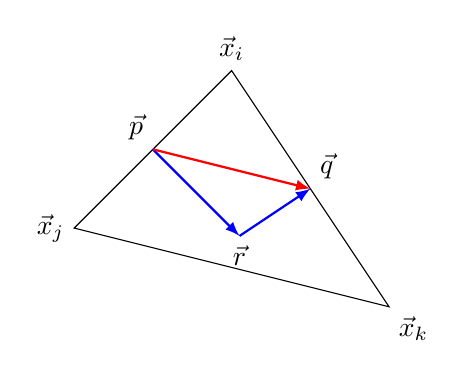
\begin{tikzpicture}
            \draw (2,3) node[above]{$\vec{x}_i$} -- (0,1) node[left]{$\vec{x}_j$} -- (4,0) node[below right]{$\vec{x}_k$} -- cycle;
            \draw[thick,blue,-latex] (1,2) --(2.1,0.9);
            \draw[thick,blue,-latex] (2.1,0.9)--(3,1.5);
            \node at (1,2) [above left]{$\vec{p}$};
            \node at (3,1.5) [above right]{$\vec{q}$};
            \node at (2.1,0.9) [below]{$\vec{r}$};
            \draw[thick,red,-latex] (1,2)--(3,1.5);
        \end{tikzpicture}
        \caption{$\p\Omega(\vec{x}_i)$在$T_m$中的一段(图中的蓝色有向线段)}
    \end{figure}
    \indent 在梯度一节中我们已经证明$\nabla f$在给定三角形上是定值,于是依照上图有
    \[\int_{\p\Omega(\vec{x}_i)\cap T_m}\nabla f\cdot\vec{n}\di s=\nabla f\cdot\int_{\p\Omega(\vec{x}_i)}\vec{n}\di s=\nabla f\cdot\left(\int_{PR}\vec{n}\di s+\int_{RQ}\vec{n}\di s\right)\]
    而对于有向线段$PR$而言,其方向向量为$\vec{t}=\dfrac{\vec{r}-\vec{p}}{||\vec{r}-\vec{p}||}$,于是
    \[\int_{PR}\vec{n}\di s=\int_{PR}\left(-\vec{t}^\bot\right)\di s=\dfrac{\left(\vec{p}-\vec{r}\right)^\bot}{||\vec{r}-\vec{p}||}\cdot\int_{PR}\di s=(\vec{p}-\vec{r})^\bot\]
    同理有$\displaystyle\int_{RQ}\vec{n}\di s=(\vec{r}-\vec{q})^\bot$.于是
    \[\int_{\p\Omega(\vec{x}_i)\cap T_m}\nabla f\cdot\vec{n}\di s=\nabla f\cdot\left((\vec{p}-\vec{r})^\bot+(\vec{r}-\vec{q})^\bot\right)=\nabla f\cdot(\vec{p}-\vec{q})^\bot\]
    按照\tbf{局部平均区域}一节中所述的$\Omega\left(\vec{x}_i\right)$的取法,$\vec{p}$和$\vec{q}$分别为各自边的中点.于是
    \[\int_{\p\Omega(\vec{x}_i)\cap T_m}\nabla f\cdot\vec{n}\di s=\dfrac12\nabla f\cdot\left(\vec{x}_j-\vec{x}_k\right)^\bot\]
    现在再将\footnote{为了简洁考虑,记$f$在$\vec{x}_i$处的值为$f_i$,其余类似}上一节中推导的梯度公式变形可得
    \[\nabla f=\left(f_j-f_i\right)\dfrac{\left(\vec{x}_i-\vec{x}_k\right)^\bot}{2A_m}+\left(f_k-f_i\right)\dfrac{\left(\vec{x}_j-\vec{x}_i\right)^\bot}{2A_m}\]
    代入上式可得
    \[\begin{aligned}
        \int_{\p\Omega(\vec{x}_i)\cap T_m}\nabla f\cdot\vec{n}\di s
        &=\dfrac{1}{4A_m}\left[\left(f_j-f_i\right)\left(\vec{x}_i-\vec{x}_k\right)^\bot\left(\vec{x}_j-\vec{x}_k\right)^\bot+\left(f_k-f_i\right)\left(\vec{x}_j-\vec{x}_i\right)^\bot\left(\vec{x}_j-\vec{x}_k\right)^\bot\right] \\
        &= \dfrac{1}{4A_m}\left[\left(f_j-f_i\right)\left(\vec{x}_i-\vec{x}_k\right)\cdot\left(\vec{x}_j-\vec{x}_k\right)+\left(f_k-f_i\right)\left(\vec{x}_i-\vec{x}_j\right)\cdot\left(\vec{x}_k-\vec{x}_j\right)\right]
    \end{aligned}\]
    上面的式子中恰好存在边的点乘与面积之比,因此考虑用三角函数表示.事实上,对于任意的$\triangle ABC$总有
    \[\dfrac{\overrightarrow{AB}\cdot\overrightarrow{AC}}{A_{\triangle ABC}}=\dfrac{\overline{AB}\cdot\overline{AC}\cdot\cos A}{\dfrac12\overline{AB}\cdot\overline{AC}\cdot\sin A}=2\cot A\]
    于是把这一结论运用到上式即可得
    \[\int_{\p\Omega(\vec{x}_i)\cap T_m}\nabla f\cdot\vec{n}\di s=\dfrac12\left[\left(f_j-f_i\right)\cot\gamma_k+\left(f_k-f_i\right)\cot\gamma_j\right]\]
    其中$\gamma_j$和$\gamma_k$分别是顶点$\vec{x}_j$和$\vec{x}_k$处的角.现在,我们将$\p\Omega(\vec{x}_i)$在所有邻接三角形中的部分累加起来,即可得
    \[\int_{\p\Omega(\vec{x}_i)}\nabla f\cdot\vec{n}\di s=\dfrac{1}{2}\sum_{j\in\Omega(i)}\left(\cot\alpha_{ij}+\cot\beta_{ij}\right)\left(f_j-f_i\right)\]
    其中$\alpha_{ij}$和$\beta_{ij}$是与边$(\vec{x}_i,\vec{x}_j)$相邻的两个三角形中该边所对的角.最后,我们只需要将上式除以邻域$\Omega(\vec{x}_i)$的面积$A(\vec{x}_i)$即可得到余切Laplacian的定义,即
    \[\Delta f\left(x_i\right)=\dfrac{1}{2A(\vec{x}_i)}\sum_{j\in\Omega(i)}\left(\cot\alpha_{ij}+\cot\beta_{ij}\right)\left(f_j-f_i\right)\]
    在实际应用中,由于$A(\vec{x}_i)$是定值,因此我们通常令权重$w_{ij}$为
    \[w_{ij}=\dfrac12\left(\cot\alpha_{ij}+\cot\beta_{ij}\right)\]
    后进行归一化处理.\\
    \indent 对权值进行简化,我们可以得到均匀Laplacian的定义.均匀Laplacian的计算量较小,但没有恰当的几何意义,在很多时候也经常导致问题.
\end{proof}
\subsection{网格平滑}
随着三维扫描和曲面重建技术的发展,得到实体表面的多边形网格表示已经不是难事,但所得到的表面往往包含噪声.为了将其转化为更光滑的网格以便后续处理,我们需要用到\tbf{网格平滑}技术.
\begin{definition}[网格平滑]
    \tbf{网格平滑(Mesh Smoothing)}(又称为\tbf{网格降噪(Mesh Deinoising)}通过)对多边形网格进行处理,以减少噪声,从而得到更光滑,性质更优良的网格表示.
\end{definition}
一般而言,噪声所在的位置都是曲率较大,形状比较尖锐的地方.因此,网格平滑的目标是减少这些高频噪声,同时尽可能地保留网格的整体形状和细节.\\
\indent 我们在本节主要介绍\tbf{拉普拉斯平滑(Laplacian Smoothing)}.\\
\indent 我们用扩散流的数学模型来描述网格平滑的过程.考虑热量传导的物理模型,设$f(\vec{x},t)$表示时间$t$时刻位置$\vec{x}$处的温度,则扩散方程为:
\[\dfrac{\p f(\vec{x},t)}{\p t}=\lambda\Delta f(\vec{x},t)\]
在网格中,高频的噪声就对应于杂乱分布的高温点.随着扩散的进行,热量分布趋于均匀,对应顶点构成的表面也趋于平滑.\\
\indent 现在,我们需要将扩散流公式在时间和空间上进行离散化,以便在计算机中处理.在空间上的Laplacian离散化已经在前面一节中介绍,即
\[\dfrac{\p f\left(\vec{x}_i,t\right)}{\p t}=\lambda\Delta f\left(\vec{x}_i,t\right)=\lambda\sum_{\vec{x}_j\in\Omega\left(\vec{x}_i\right)}w_{ij}\left(f\left(\vec{x}_j,t\right)-f\left(\vec{x}_i,t\right)\right)\]
而在时间上的离散化,可以将$t$划分为步长为$h$的若干个间隔,用有限差分的思想对微分方程进行近似:
\[\dfrac{\p f\left(\vec{x}_i,t\right)}{\p t}=\dfrac{f\left(\vec{x}_i,t+h\right)-f\left(\vec{x}_i,t\right)}{h}\]
于是
\[f\left(\vec{x}_i,t+h\right)=f\left(\vec{x}_i,t\right)+h\dfrac{\p f\left(\vec{x}_i,t\right)}{\p t}=f\left(\vec{x}_i,t\right)+h\lambda\sum_{\vec{x}_j\in\Omega\left(\vec{x}_i\right)}w_{ij}\left(f\left(\vec{x}_j,t\right)-f\left(\vec{x}_i,t\right)\right)\]
\indent 在网格简化中,我们考虑的``温度''就是顶点的空间坐标.于是,在每次时间间隔为$h$的第$k$次迭代中,每个顶点$\vec{x}_i$的位置按照如下的方式更新:
\[\vec{x}_i^{(k+1)}\leftarrow\vec{x}_i^{(k)}+\lambda\Delta\vec{x}_i^{(k)}\]
其中$\lambda$为\tbf{平滑参数}即为前面推导中的$h\lambda$.\\
\indent 在两种Laplacian下,上述迭代方法可以得到不同的平滑效果.均匀Laplacian下,每个顶点都向其邻居的均值移动,这种方法简单且计算效率高,但容易导致网格收缩和细节丢失.余切Laplacian下,每个顶点向平均曲率的方向移动,也被称作\tbf{平均曲率流(Mean Curvature Flow)}.这种方法能够更好地保留网格的形状和细节,但是计算复杂度较高.
\subsection{网格编辑}
\begin{definition}[网格编辑]
    \tbf{网格编辑(Mesh Editing)}是操纵和修改网格表面的几何形状,同时能够保留原始网格几何细节的操作.
\end{definition}
回顾我们对二维图像进行Poisson编辑的过程,这可以描述为下面的最小化问题:
\[\arg\min_{f}\iint_{\Omega}\left|\left|\nabla f-\nabla g\right|\right|^2\di S,\quad\text{s.t.}\quad f|_{\p\Omega}=f^\ast|_{\p\Omega}\]
类似的思想在三维情形下的应用就是Laplacian网格编辑.它通过尽可能使得编辑后网格上的Laplace微分坐标与原始网格上的Laplace微分坐标保持一致保留网格的细节. Laplace微分坐标在本质上就是对网格顶点施加均匀Laplacian的结果,即
\[\mathcal{L}\left(\vec{v}_i\right)=\vec{v}_i-\dfrac{1}{N_i}\sum_{j\in\Omega(i)}\vec{v}_j\]

\subsection{网格简化}
在图形学中,渲染效率与渲染质量需要兼顾.同样的物体在近处时需要使用精度较高,面数较多的模型以保证真实;而在远处时由于物体在屏幕上占据的像素较少,使用精度较低,面数较少的模型也能保证视觉效果.因此,我们需要对高精度的网格进行简化以提高渲染效率.这时就需要用到\tbf{网格简化}算法来生成不同\tbf{细节层次(Level of Detail, LoD)}的模型用于不同情况下的渲染.
\begin{definition}
    \tbf{网格简化(Mesh Simplification)}通过对多边形网格进行处理,以减少其面数,从而得到更简洁,渲染效率更高的网格表示.
\end{definition}
网格简化一般可以通过移除顶点或坍缩边实现,实际应用中后者更容易实现,也更常用.边坍缩算法的核心是设计方法找出哪些边的坍缩对网格形状的影响最小,以及确定坍缩后新顶点的位置,从而在简化时尽量保留网格的整体形状.\\
\indent 我们在本节主要介绍\tbf{二次误差度量(Quadric Error Metrics, QEM)}方法\footnote{Garland M, Heckbert PS. Surface simplification using quadric error metrics. In: Proceedings of the 24th annual conference on computer graphics and interactive techniques. 1997, p. 209-16.}.对于一次边坍缩,考虑将$\vec{v}_1,\vec{v}_2$收缩为$\vec{v}$.为了度量收缩操作与原网格的差异,我们可以用简化后的点与原网格中$\vec{v}_1,\vec{v}_2$邻接的所有面的距离之和来表示.\\
\indent 定义$\text{plain}\left(\vec{v}_i\right)$表示所有与顶点$\vec{v}_i$邻接的面的集合,其中的元素$\vec{p}=\begin{bmatrix}
    a&b&c&d
\end{bmatrix}^{\text{t}}$表示对应平面的方程为$ax+by+cz+d=0$,并且$a^2+b^2+c^2=1$.于是优化目标为:
\[\vec{v}^\ast=\arg\min_{\vec{v}}\sum_{\vec{p}\in\text{plain}\left(\vec{v}_1\right)\cup\text{plain}\left(\vec{v}_2\right)}d_{\vec{v},\vec{p}}^2\]
在这里,为了计算方便,我们将$\vec{v}$扩展为具有四个分量的向量$\vec{v}=\begin{bmatrix}
    x&y&z&1
\end{bmatrix}^{\text{t}}$,其中前三个分量表示$\vec{v}$的位置.于是点$\vec{v}$到平面$\vec{p}$的距离为:
\[d_{\vec{v},\vec{p}}^2=\left(\vec{v}^{\text{t}}\vec{p}\right)^2=\vec{v}^{\text{t}}\vec{p}\vec{p}^{\text{t}}\vec{v}\]
令$\mat{K}_{\vec{p}}=\vec{p}\vec{p}^{\text{t}}$,则有
\[\vec{v}^\ast=\arg\min_{\vec{v}}\vec{v}^{\text{t}}\left(\sum_{\vec{p}\in\text{plain}\left(\vec{v}_1\right)\cup\text{plain}\left(\vec{v}_2\right)}\mat{K}_{\vec{p}}\right)\vec{v}\]
为了简化计算,我们将上式近似为
\[\vec{v}^\ast=\arg\min_{\vec{v}}\vec{v}^{\text{t}}\left(\sum_{\vec{p}\in\text{plain}\left(\vec{v}_1\right)}\mat{K}_{\vec{p}}+\sum_{\vec{p}\in\text{plain}\left(\vec{v}_2\right)}\mat{K}_{\vec{p}}\right)\vec{v}\]
实际上至多只会重复以$\vec{v}_1,\vec{v}_2$为顶点的两个三角形面,但将误差转化为仅与顶点相关的信息,因而简化了计算.令$\mat{Q}_i=\displaystyle\sum_{\vec{p}\in\text{plain}\left(\vec{v}_i\right)}\mat{K}_{\vec{p}}$,于是就有
\[\vec{v}^\ast=\arg\min_{\vec{v}}\vec{v}^{\text{t}}\left(\mat{Q}_1+\mat{Q}_2\right)\vec{v}\]
现在来考虑这一二次型的最小值何时取到.令$\mat{Q}=\mat{Q}_1+\mat{Q}_2$,将上述式子展开可得
\[\vec{v}^{\text{t}}\mat{Q}\vec{v}=q_{11}x^2+2q_{12}xy+2q_{13}xz+2q_{14}x+q_{22}y^2+2q_{23}yz+2q_{24}y+q_{33}z^2+2q_{34}z+q_{44}\]
并且要求
\[\dfrac{\p\vec{v}^{\text{t}}\mat{Q}\vec{v}}{\p x}=\dfrac{\p\vec{v}^{\text{t}}\mat{Q}\vec{v}}{\p y}=\dfrac{\p\vec{v}^{\text{t}}\mat{Q}\vec{v}}{\p z}=0\]
于是可以得到如下线性方程组:
\[\begin{bmatrix}
    q_{11}&q_{12}&q_{13}&q_{14}\\
    q_{21}&q_{22}&q_{23}&q_{24}\\
    q_{31}&q_{32}&q_{33}&q_{34}\\
    0&0&0&1
\end{bmatrix}\begin{bmatrix}
    x\\y\\z\\1
\end{bmatrix}=\begin{bmatrix}
    0\\0\\0\\1
\end{bmatrix}\]
令$\mat{Q}'$为前面的矩阵,则有$\mat{Q}'\vec{v}^\ast=\begin{bmatrix}
    0&0&0&1
\end{bmatrix}^{\text{t}}$.如果$\mat{Q}'$可逆,就有
\[\vec{v}^\ast=\left(\mat{Q}'\right)^{-1}\begin{bmatrix}
    0&0&0&1
\end{bmatrix}^{\text{t}}\]
如果$\mat{Q}'$不可逆,这就说明我们无法找出使误差最小的$\vec{v}$.此时,我们可以简单地选择$\vec{v}_1,\vec{v}_2$以及它们的中点$\dfrac{\vec{v}_1+\vec{v}_2}{2}$中使得误差$\vec{v}^{\text{t}}\mat{Q}\vec{v}$最小的点作为优化的结果$\vec{v}^\ast$.需要注意的是,这里的$\mat{Q}'$\textit{仅作为}求解$\vec{v}^\ast$使用.计算误差仍然使用$\mat{Q}$.\\
\indent 于是, QEM算法的基本流程为:
\begin{enumerate}[label=\tbf{\arabic*.},topsep=0pt,parsep=0pt,itemsep=0pt,partopsep=0pt]
    \item 初始化每个顶点的误差矩阵$\mat{Q}_i$.
    \item 对每组合法的(可收缩而不改变网格拓扑结构的)点对$(\vec{v}_1,\vec{v}_2)$,计算其误差矩阵$\mat{Q}=\mat{Q}_1+\mat{Q}_2$以及最优收缩点$\vec{v}^\ast$和误差$\text{err}(\vec{v}^\ast)=\left(\vec{v}^\ast\right)^{\text{t}}\mat{Q}\vec{v}^\ast$.
    \item 将所有点对按误差从小到大存入优先队列中.
    \item 重复以下操作直到达到预定的顶点数:
    \begin{enumerate}[label=\tbf{\alph*.},topsep=0pt,parsep=0pt,itemsep=0pt,partopsep=0pt]
        \item 从优先队列中取出误差最小的点对$(\vec{v}_1,\vec{v}_2)$,并将其坍缩为$\vec{v}^\ast$,在网格结构中实现这一操作.
        \item 考虑所有坍缩前与$\vec{v}_1,\vec{v}_2$相邻的顶点$\vec{u}_1,\cdots,\vec{u}_n$.首先,由于$\vec{u}_i$相邻的点已经更新为$\vec{v}^\ast$,因此其相邻的面已经发生改变,因此需要重新计算$\vec{u}_i$的误差矩阵.然后考虑所有与$\vec{u}_i$相邻的顶点$\vec{w}_{i1},\cdots,\vec{w}_{im}$,对于顶点对$\left(\vec{u}_i,\vec{w}_{ij}\right)$,由于$\vec{u}_i$的误差矩阵发生变化,因此需要重新判断点对是否合法,并重新计算收缩点和误差,最后将其更新到优先队列中.
    \end{enumerate}
\end{enumerate}
\end{document}